\documentclass{article}
\usepackage{amsmath}
\usepackage{tikz} 
\usepackage[a4paper]{geometry}
\usepackage{fancyhdr}
\pagestyle{fancy}
\lhead{Vektorprodukte}
\rhead{Juni 2025}
\begin{document}
  
\newcommand{\norm}[1]{\big| {#1} \big|}  
\newcommand{\vect}[1]{\overrightarrow{#1}} 
 
\section{Vektorprodukte} 
\begin{minipage}{\dimexpr\textwidth-4cm} 
Das \emph{Vektorenprodukt}, auch \emph{Kreuzprodukt} genannt, von zwei Vektoren $\vect{a}$ und $\vect{b}$ ist ein anderer Vektor, genannt der \emph{Lotvektor} oder \emph{Normalvektor}, welcher zu beiden Vektoren orthogonal ist. Somit ist $\vect{a} \times \vect{b} = \vect{n}$, wenn $\vect{n} \cdot \vect{a} = 0$ und $\vect{n} \cdot \vect{b} = 0$ ist. Dabei dürfen $\vect{a}$ und $\vect{b}$ nicht kollinear sein. \newline
Es gilt 
\[
 \vect{a} \times \vect{b} =
 \begin{pmatrix}
  a_2 \cdot b_3 - a_3 \cdot b_2 \\
  a_3 \cdot b_1 - a_1 \cdot b_3 \\
  a_1 \cdot b_2 - a_2 \cdot b_1 
 \end{pmatrix}
\]
\end{minipage} 
\hfill
\begin{minipage}{4cm}
 \centering 
 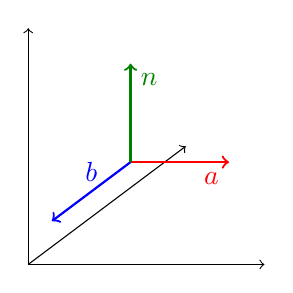
\begin{tikzpicture} 
  \draw[->] (0,0) -- (3,0);
  \draw[->] (0,0) -- (0,3);
  \draw[->] (0,0) -- (2,1.5); 
 
  \draw[thick,blue,->] (1.3,1.3) -- ++(-1,-1*0.75) node[midway, above] {$\vect{b}$};
  \draw[thick,red,->] (1.3,1.3) -- ++(1.25,0) node[below left] {$\vect{a}$};
  \draw[thick,green!50!black,->] (1.3,1.3) -- ++(0,1.25) node[below right] {$\vect{n}$};
 \end{tikzpicture}
\end{minipage} 
  
\vspace{1em} \noindent
\begin{minipage}{3cm}
 \centering 
 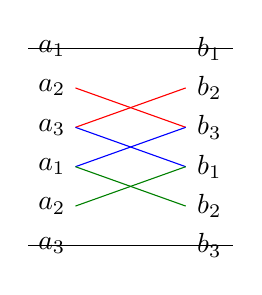
\begin{tikzpicture}
  \node at (0,0) {$a_1$};
  \node at (0,-0.5) {$a_2$};
  \node at (0,-1) {$a_3$};
  \node at (0,-1.5) {$a_1$};
  \node at (0,-2) {$a_2$};
  \node at (0,-2.5) {$a_3$}; 
 
  \node at (2,0) {$b_1$};
  \node at (2,-0.5) {$b_2$};
  \node at (2,-1) {$b_3$};
  \node at (2,-1.5) {$b_1$};
  \node at (2,-2) {$b_2$};
  \node at (2,-2.5) {$b_3$};
 
  \draw[black] (-0.3,0) -- (2.3,0); 
  \draw[black] (-0.3,-2.5) -- (2.3,-2.5);
  \draw[red] (0.3,-0.5) -- (1.7,-1);
  \draw[red] (0.3,-1) -- (1.7,-0.5);
  \draw[blue] (0.3,-1) -- (1.7,-1.5);
  \draw[blue] (0.3,-1.5) -- (1.7,-1);
  \draw[green!50!black] (0.3,-1.5) -- (1.7,-2);
  \draw[green!50!black] (0.3,-2) -- (1.7,-1.5);
 \end{tikzpicture}  
\end{minipage} 
\hfill
\begin{minipage}{\dimexpr\textwidth-3cm}
Eine Eselsbrücke ist es dabei die Vektoren zweimal untereinander aufzuschreiben, die oberste und unterste Reihe zu ignorieren und dann in der Diagonale zu multiplizieren. \newline
So wird, mit $a_2$ angefangen, hochgezählt drei mal mit dem nächsten $b$ des nächsten Indexes multipliziert, wovon das Produkt der gleichen Indexes, mit $a$ und $b$ getauscht, abgezogen wird.
\end{minipage} 
 
 
\end{document} 
 
